\chapter{Descrizione del sistema}
\section{Raccolta dei requisiti}
I requisiti sono stati raccolti tramite le seguenti metodologie:
\begin{list}{$\cdot$}{}
    \item interview con gli stakeholder interessati (rappresentata dalla traccia testuale ai fini dell’esame).
    \item identificazione ed Analisi delle personas.
\end{list}

\subsection{Personas}
Sono state identificate quattro personas, di cui le prime due sono personas
significative per la classe dei clienti, la terza è significativa per
la classe degli agenti immobiliari, la quarta ed ultima lo è
per la classe degli amministratori.

\noindent
Dall'analisi di ciascuna persona, sono stati ricavati requisiti funzionali del sistema.

\begin{figure}[h]
    \centering
    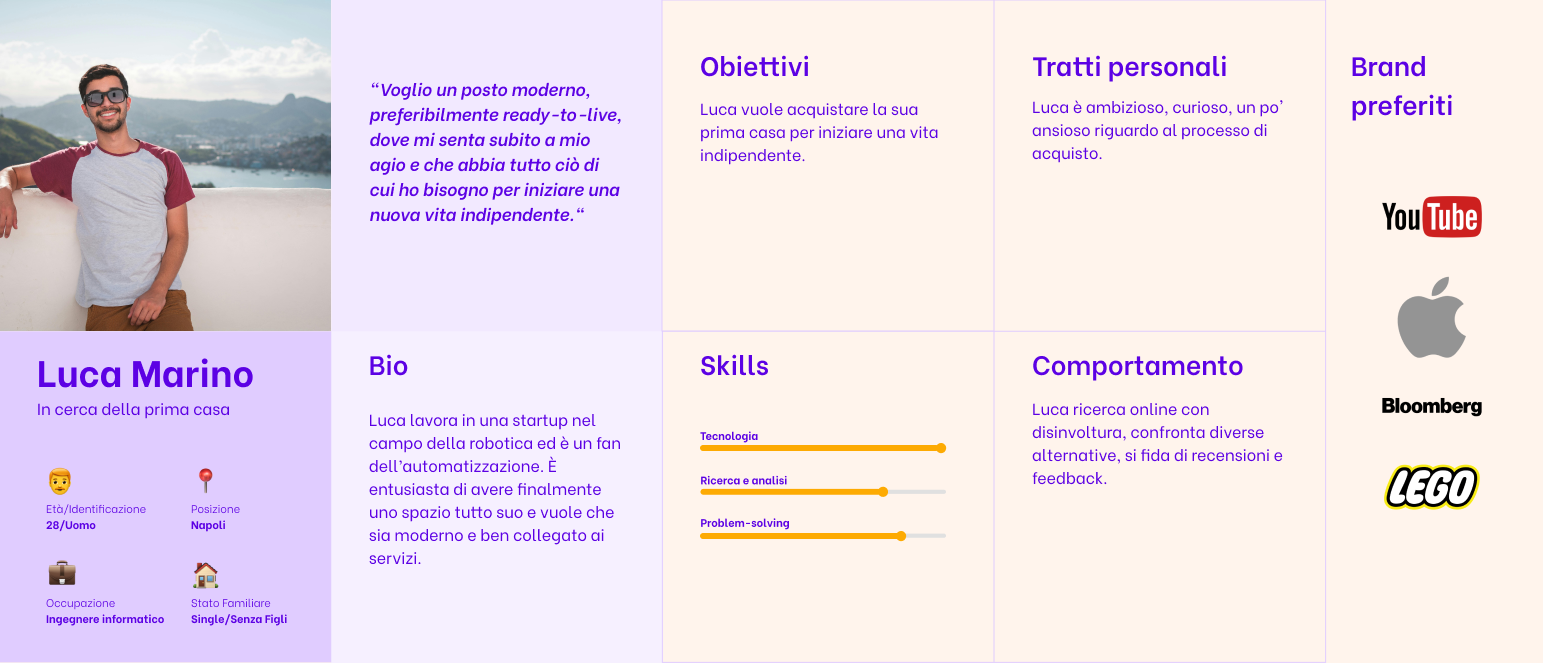
\includegraphics[width=\textwidth]{assets/personas/luca-marino.png}
    \caption{Persona: Luca Marino}
    \label{fig:luca-marino}
\end{figure}

\noindent
Dall'analisi di Luca, si evince che il sistema deve:
\begin{list}{$\cdot$}{}
    \item permettere di comunicare con l’agente online, senza telefonate.
    \item permettere di visualizzare valutazioni/recensioni degli agenti immobiliari.
\end{list}

\begin{figure}[h]
    \centering
    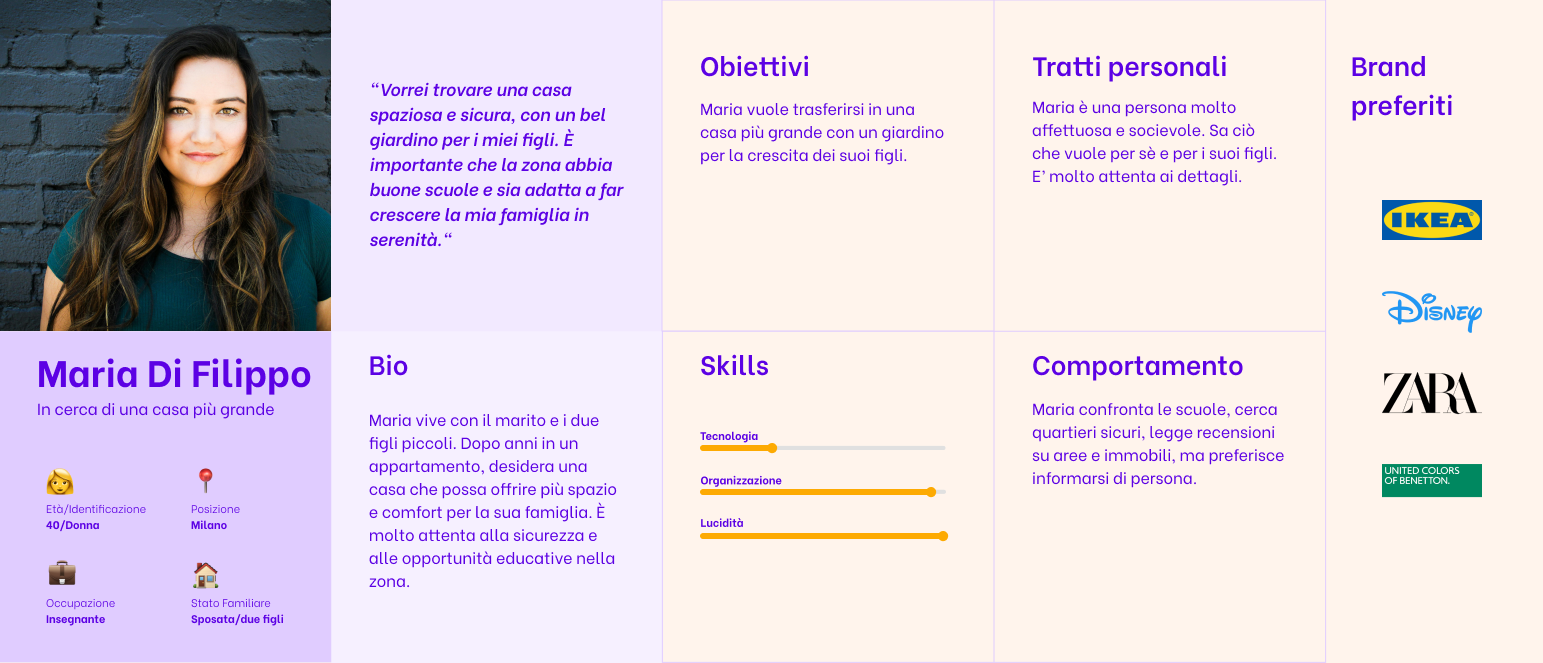
\includegraphics[width=\textwidth]{assets/personas/maria-di-filippo.png}
    \caption{Persona: Maria Di Filippo}
    \label{fig:maria-di-filippo}
\end{figure}

\noindent
Dall'analisi di Maria, si evince che il sistema deve:
\begin{list}{$\cdot$}{}
    \item presentare un'interfaccia rifinita per veicolare professionalità.
    \item permettere di telefonare l'agente immobiliare.
    \item permettere di visualizzare parchi, scuole nella mappa interattiva (verrà supportato in futuro).
\end{list}

\begin{figure}[h]
    \centering
    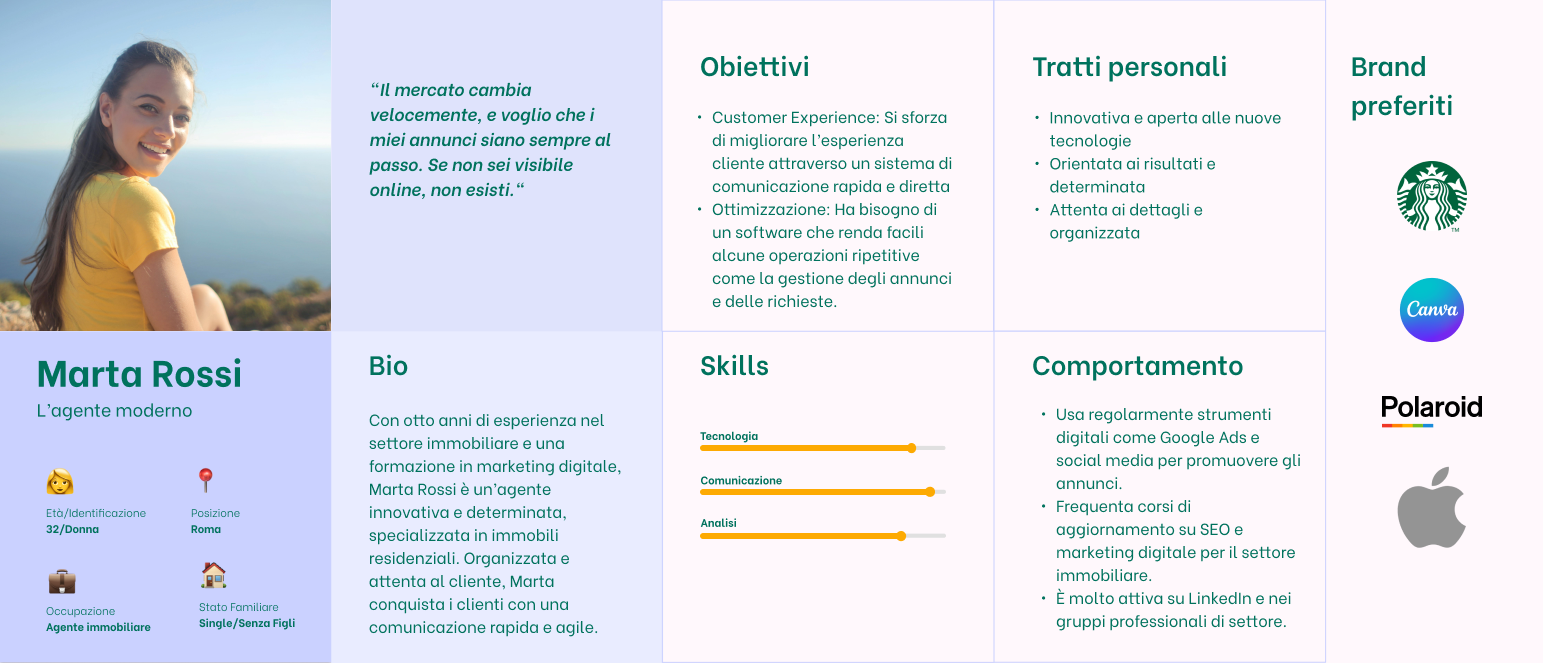
\includegraphics[width=\textwidth]{assets/personas/marta-rossi.png}
    \caption{Persona: Marta Rossi}
    \label{fig:marta-rossi}
\end{figure}

\noindent
Dall'analisi di Marta, si evince che il sistema deve:
\begin{list}{$\cdot$}{}
    \item permettere di descrivere dettagli di un immobile in fase di creazione/modifica dell'annuncio.
    \item permettere di personalizzare il profilo di un agente.
    \item essere efficiente nella gestione di annunci, messaggi, richieste di visite.
    \item permettere di analizzare i risultati ottenuti mediante una dashboard (verrà supportato in futuro).
\end{list}

\begin{figure}[h]
    \centering
    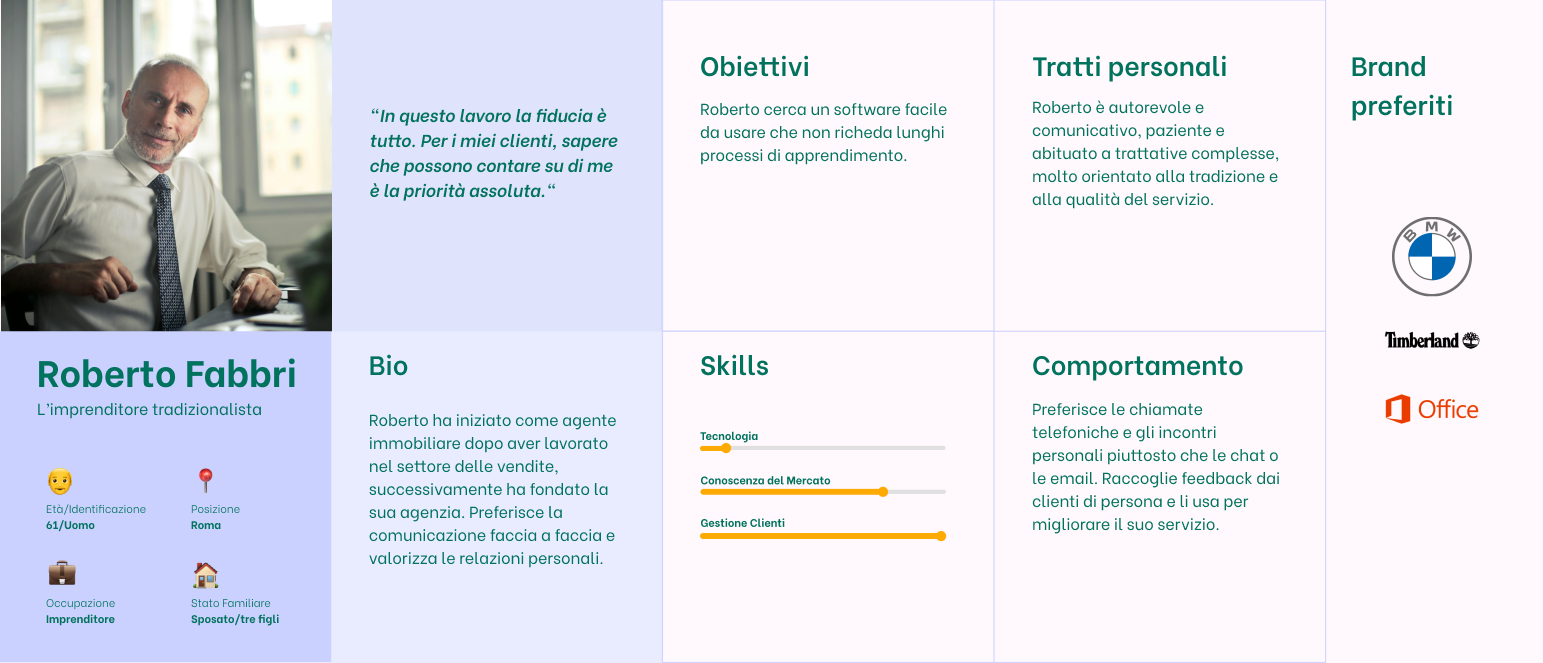
\includegraphics[width=\textwidth]{assets/personas/roberto-fabbri.png}
    \caption{Persona: Roberto Fabbri}
    \label{fig:roberto-fabbri}
\end{figure}

\noindent
Dall'analisi di Roberto, si evince che il sistema deve:
\begin{list}{$\cdot$}{}
    \item avere un'interfaccia usabile sin dalle prime esperienze.
    \item permettere di telefonare l'agente immobiliare.
    \item di analizzare feedback lasciati dai clienti mediante una dashboard (verrà supportato in futuro).
\end{list}

\begin{figure}[h]
    \centering
    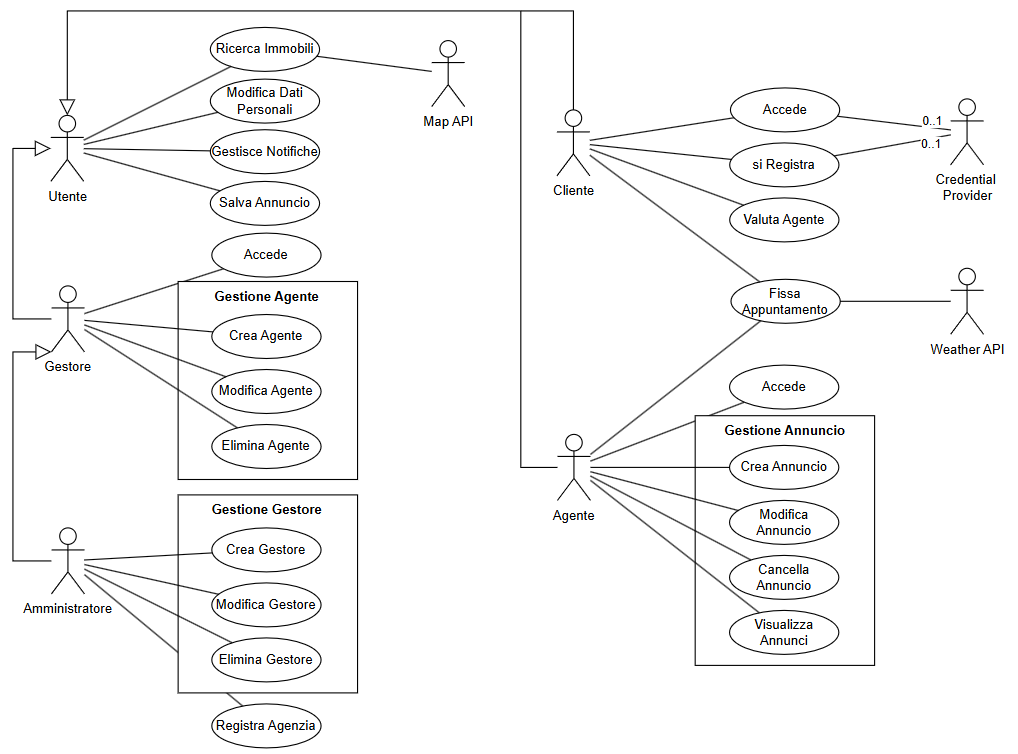
\includegraphics[width=\textwidth]{assets/diagrams/use-case-diagram.png}
    \caption{Use case diagram}
    \label{fig:use-case-diagram}
\end{figure}

\section{Requisiti funzionali}
% Descrizioni brief degli use case
Per ogni use case individuato, si fornisce in questa sezione una
specifica di tipo brief.
I requisiti funzionali verranno raggruppati secondo
classi di utenti: utente, gestore, amministratore, cliente.

\subsection{Utente}
\subsubsection{Ricerca Immobili}
L'utente ricerca immobili tramite l'apposita barra, può ricercare 
immobili da affittare o da acquistare. É possibile ricercare 
l'immobile utilizzando diversi filtri. il sistema mostra i risultati ottenuti.

\subsubsection{Modifica dati personali}
L'utente accede alla schermata di visualizzazione dei dati personali, modifica 
i campi del form predisposti alla modifica e una volta finito clicca su salva. 
Il sistema salva le modifiche.

\subsubsection{Gestisci notifiche}
L'utente accede alla schermata di gestione delle notifiche, dove
può modificare la modalità di ricezione delle notifiche, organizzate 
in categorie, tramite appositi pulsanti. L'utente conferma le modifiche. 
Il sistema tiene traccia delle modifiche.

\subsubsection{Salva Annuncio}
L'utente, una volta visualizzati i risultati di una ricerca di immobili,
clicca sul pulsante a forma di stella. Il sistema tiene traccia
dell'operazione.

\subsection{Gestore}
\subsubsection{Accede}
Il gestore accede alla schermata per l'accesso ed inserisce le credenziali, 
accedendo così alla schermata principale per i gestori. Il sistema tiene 
traccia dell'accesso.

\subsubsection{Crea Agente}
Il gestore accede alla schermata di creazione di un agente, inserisce i 
dati necessari e conferma. Il sistema crea un nuovo utente Agent.

\subsubsection{Modifica Agente}
Il gestore accede alla schermata di gestione degli agenti, da cui 
seleziona un agente per la modifica. Il sistema tiene traccia delle
modifiche.

\subsubsection{Elimina Agente}
Il gestore accede alla schermata di gestione degli agenti, da cui 
seleziona un agente per la sua eliminazione. Il sistema tiene traccia delle
modifiche.

\subsection{Amministratore}
\subsubsection{Crea Gestore}
L'Amministratore accede alla schermata di creazione di un gestore, 
inserisce i dati necessari e conferma. Il sistema crea un nuovo utente Manager.

\subsubsection{Modifica Gestore}
L'amministratore accede alla schermata di gestione dei gestori, da cui 
seleziona un gestore per la modifica. Il sistema tiene traccia delle
modifiche.

\subsubsection{Elimina Gestore}
L'amministratore accede alla schermata di gestione dei gestori, da cui 
seleziona un gestore per l'eliminazione. Il sistema tiene traccia delle
modifiche.

\subsubsection{Registra Agenzia}
L'amministratore, non ancora registrato al sistema, accede alla schermata di registrazione 
ed inserisce i propri dati e i dati dell'agenzia immobiliare. Il sistema registra l'agenzia 
e crea un utente Admin per l'amministratore.

\subsection{Cliente}
\subsubsection{si Registra}
L'utente accede alla schermata per la registrazione, si registra inserendo
i dati necessari oppure tramite un credential provider esterno. 
Il sistema crea un utente Client.

\subsubsection{Accede}
L'utente accede alla schermata per l'accesso ed inserisce le credenziali 
compilando il form di accesso oppure utilizzando un credential provider esterno. 
Il sistema mostra la schermata principale di ricerca e tiene traccia 
dell'avvenuto accesso.

\subsubsection{Valuta Agente}
L'utente, nella schermata dell'annuncio selezionato, valuta, con un voto da 1 
a 5, l'agente immobiliare che relativo all'annuncio.

\subsubsection{Fissa Appuntamento (dal punto di vista del Cliente)}
Un cliente, dalla schermata dettagliata dell'annuncio selezionato, clicca sul 
pulsante “Richiedi Appuntamento”. Il sistema mostra una nuova schermata in cui il 
cliente puó specificare le proprie disponibilità (giorni, fasce orarie). 
Dopodiché, il cliente invia la richiesta di appuntamento. Il sistema tiene
traccia della richiesta e notifica l'agente.

\subsection{Agente}
\subsubsection{Accede}
L'utente accede alla schermata per l'accesso ed inserisce le credenziali 
compilando il form di accesso. Il sistema mostra la schermata principale 
e tiene traccia dell'avvenuto accesso.

\subsubsection{Modifica dati personali}
L'agente, dalla sua schermata principale, accede alla schermata per la 
modifica dei dati personali. In questa schermata, l'agente può:
\begin{list}{$\cdot$}{}
    \item modificare la propria biografia completa,
    \item modificare la foto profilo,
    \item modificare la bio.
\end{list} 
L'agente conferma le modifiche effettuate. Il sistema tiene traccia 
delle modifiche ed fornisce un feedback all'agente.

\subsubsection{Crea Annuncio}
L'agente accede alla schermata di inserimento di un nuovo annuncio, dove 
può compilare un form che descriva l'immobile tramite le sue caratteristiche.
Una volta compilato il form, l'agente conferma l'inserzione. 
Il sistema tiene traccia dell'inserzione ed informa l'agente dell'inserimento.

\subsubsection{Visualizza Annunci}
L'agente, dalla schermata principale, clicca sul pulsante “Annunci”, accedendo 
alla schermata di visualizzazione dei propri annunci.

\subsubsection{Modifica Annuncio}
L'agente accede alla schermata di visualizzazione dei propri annunci. Dopodiché 
seleziona un annuncio per la sua modifica. Verrà mostrata il form delle 
caratteristiche già menzionato nella descrizione del caso d'uso \textit{Crea Annuncio}.

\subsubsection{Cancella Annuncio}
L'agente, nella sezione dei propri annunci, seleziona un annuncio e clicca sul 
pulsante "cancella". Il sistema tiene traccia delle modifiche.

\subsubsection{Fissa Appuntamento (dal punto di vista dell'agente)}
Un agente riceve una notifica di richiesta di visita.
La notifica contiene informazioni su giorni e fasce orarie richiesti
dal cliente.
Se l'agente clicca su "Accetta", viene mostrata la schermata di selezione 
dell'orario e del giorno (come quella dell'utente) contenente le disponibilità 
indicate dal cliente. Da questa schermata, l'agente sceglie data ed ora 
dell'appuntamento e conferma l'appuntamento, oppure clicca su "Annulla", 
tornando allo step precedente.
